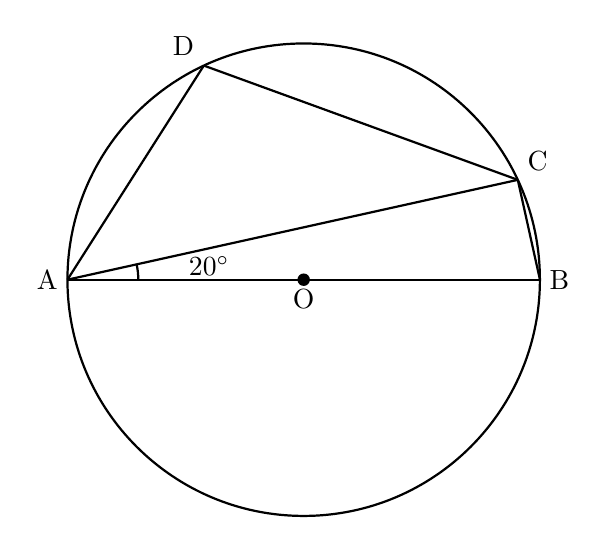
\begin{tikzpicture}[scale=1.5]

    % --- Define Coordinates ---
    % Center O at origin
    \coordinate (O) at (0,0);
    
    % Radius of the circle
    \def\R{2.0}
    
    % Point A (Left end of diameter)
    \coordinate (A) at (-\R, 0);
    
    % Point B (Right end of diameter)
    \coordinate (B) at (\R, 0);
    
    % Point C on the circle (approx 25 degrees)
    \coordinate (C) at (25:\R);
    
    % Point D on the circle (approx 115 degrees)
    \coordinate (D) at (115:\R);

    % --- Draw Circle and Center ---
    \draw[thick] (O) circle (\R);
    \fill (O) circle (1.5pt);

    % --- Draw Segments ---
    % Diameter AB
    \draw[thick] (A) -- (B);
    
    % Chords forming the polygon
    \draw[thick] (A) -- (D); % Segment AD
    \draw[thick] (D) -- (C); % Segment DC
    \draw[thick] (C) -- (B); % Segment CB
    
    % Chord AC (Diagonal)
    \draw[thick] (A) -- (C);

    % --- Angle Arc ---
    % Arc at Vertex A between line AB and AC
    % The angle is approximately 25 degrees
    \draw[thick] (A) ++(0.6,0) arc (0:13:0.6);
    
    % Label for the angle. The text in the image is handwritten/blurry, 
    % usually representing a variable like x.
    \node at (-0.8, 0.12) {$20^{\circ}$};

    % --- Point Labels ---
    \node[left] at (A) {A};
    \node[right] at (B) {B};
    \node[above right] at (C) {C};
    \node[above left] at (D) {D};
    \node[below] at (O) {O};

\end{tikzpicture}